%%%%% Section 3 A Library with Rabbit Holes %%%%%
\section{A Library with Rabbit Holes}\label{sec:framework}

Recall the visitor introduced in Section~\ref{sec:introduction}. Part of what he
wants he can clearly name---a performer (Miles Davis), a work (\textit{Kind of
    Blue}), and with them a genre (jazz)---and for that part, any catalogue serves.
The rest he could only circle with words: quiet, with feeling in it, colors
melting into one another. That part is connotative, and it belongs not to search
but to exploration. What exploration space, then, does such a visitor need? That
question is the subject of this section.

Throughout this paper, a collection is taken to give us two kinds of data:
\emph{descriptors}, the structured names carried on the bibliographic record,
and \emph{content data}, vectorial data representing the work itself, equipped
with a general-purpose inner product by which the closeness of two works is
measured. We call the pair \emph{collection data}; it is all we have to build
from. We keep, unless otherwise stated, to the simplest case, in which the only
descriptors given are genre and title.

\begin{figure}[t]
    \centering
    \begin{subfigure}{0.51\linewidth}
        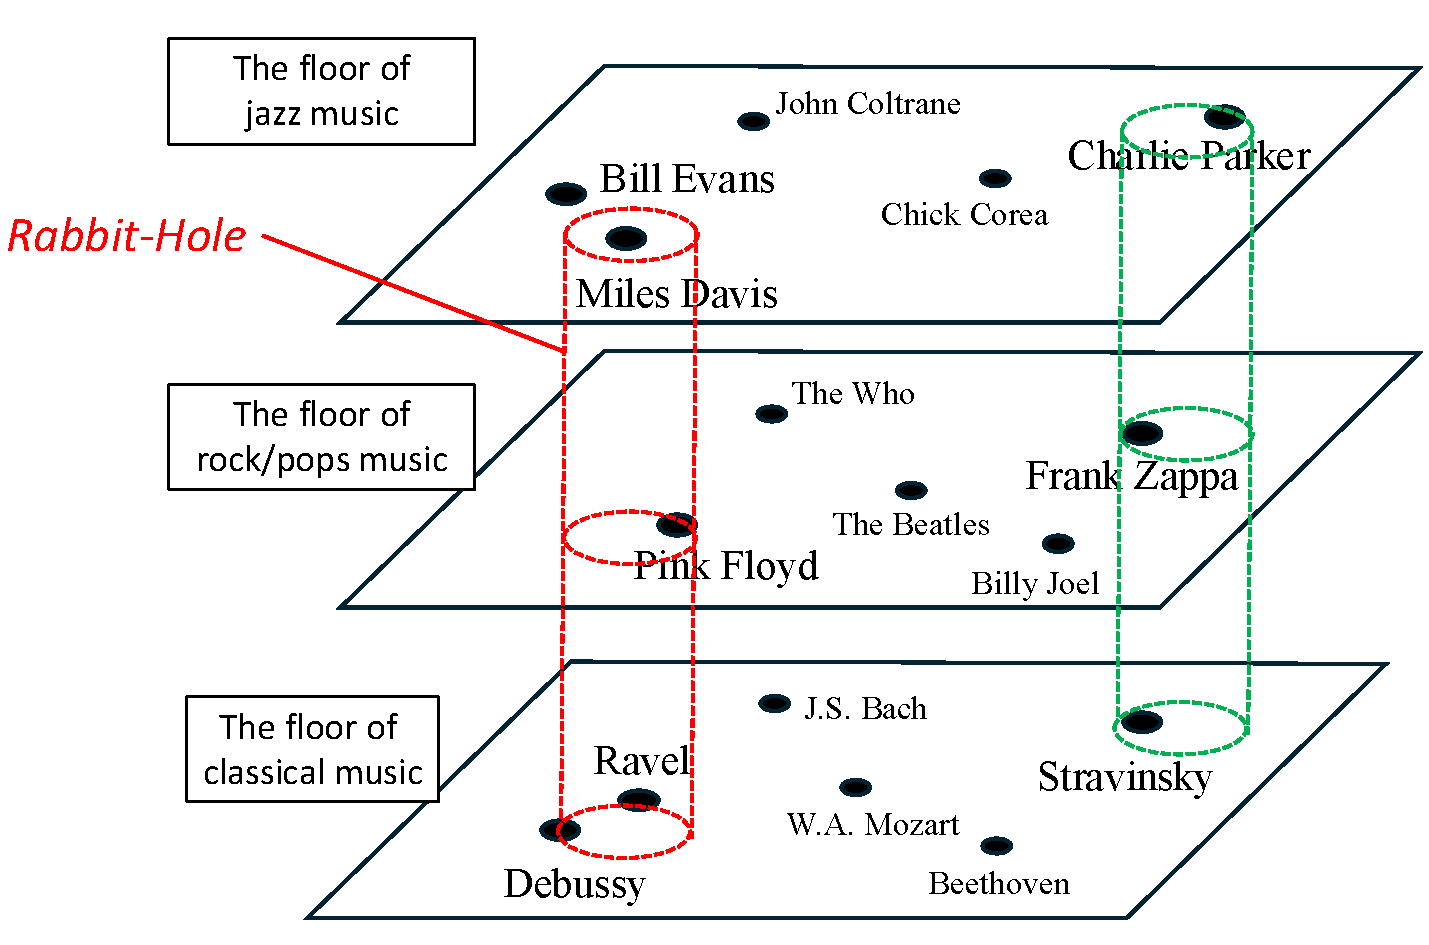
\includegraphics[width=1.0\linewidth]{fig/fig1a.pdf}
        \caption{The multi-floor library with rabbit holes (disentangled view).}
    \end{subfigure}
    \vspace{3mm}
    \begin{subfigure}{0.48\linewidth}
        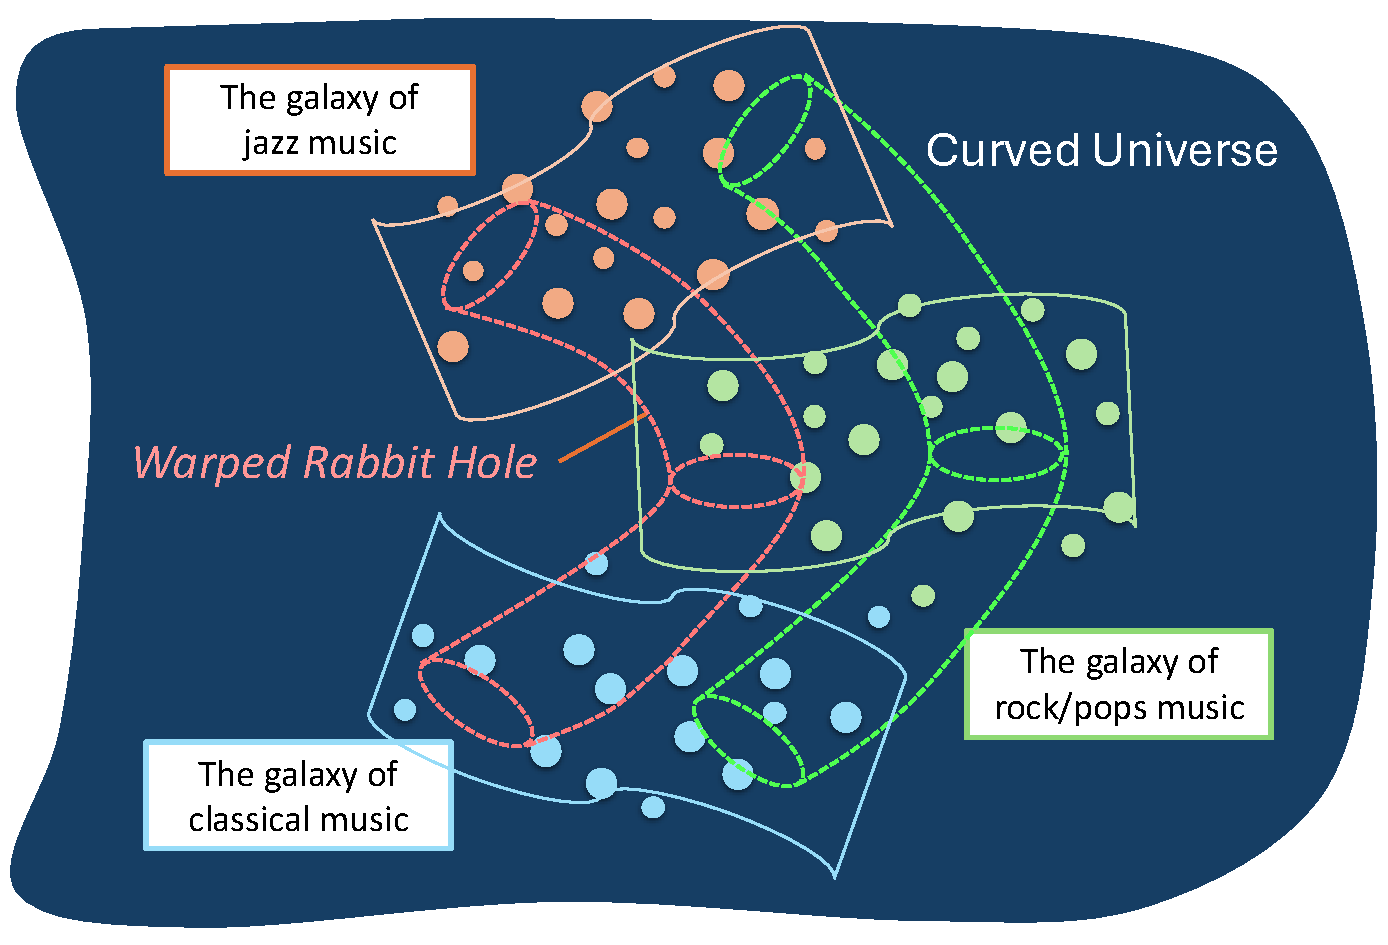
\includegraphics[width=1.0\linewidth]{fig/fig1b.pdf}
        \caption{The multi-galaxy curved universe (entangled view).}
    \end{subfigure}
    \caption{
        \textbf{Two views of one representation.}
        (a) The multi-floor library: each floor holds one genre, works
        within a floor are arranged by connotative closeness, and
        \textit{rabbit holes} run vertically, opening at the same
        connotative position on every floor. Each point is a work,
        labelled by its artist for legibility; two holes are drawn.
        (b) The same works as their native high-dimensional content
        data: each genre scatters into a loose \textit{galaxy} of its
        own, which can be modeled as a curved surface sharing no axes
        with the others; works sharing one connotation trace curved
        trajectories from galaxy to galaxy---rabbit holes in their
        entangled form.
    }
    \label{fig:two_views}
\end{figure}


%%% Subsection 3.1 The Multi-Floor Library %%%%%
\subsection{The Multi-Floor Library: The Disentangled
    Form}\label{subsec:multi_floor_library}

Consider first what descriptors alone can build: works gathered by genre, one
floor to each in a library, and within a floor shelved in title order. The
visitor asks for the jazz floor, finds Miles Davis's \textit{Kind of Blue}, and
there his intention runs out. Title order tells him nothing of what a work is
like, so he cannot move even along the jazz floor toward what he is after; on
the classical floor he can only take works down at random.

Suppose now that content data is available---acoustic features, or
whatever else can measure how near two works stand---and that each floor
is arranged by that closeness. Standing at \textit{Kind of Blue}, he
finds other Miles Davis recordings at hand, and walking on, other jazz
works of kindred sound. Along a floor, then, he can move. The same
closeness can be measured across genres too, but there it reports only
that the two stand far apart: what Miles Davis shares with Debussy is
far subtler than what separates jazz from classical. Each floor is
therefore arranged on its own lines, and no two floors agree; arriving
on the classical floor, he cannot tell where to begin.

Neither library, then, gives the visitor what he needs. Before designing
one that does, let us state what is wanted of it. Our requirements are
Bj\"orneborn's three affordances
(Section~\ref{subsec:systems})~\cite{Bjorneborn20171053}, restated as
conditions on a representation, joined by a fourth of our own.
%
\begin{itemize}
    \item \textbf{(R1) Sensible in place:} standing anywhere in the
          space, the visitor can feel the texture of the works around
          him and sense where he is.
    \item \textbf{(R2) Diverse in direction:} the space offers him many
          directions to differ along.
    \item \textbf{(R3) Traversable at will:} he can choose his own
          direction and move through the space as he pleases.
    \item \textbf{(R4) Foreseeable in direction:} he can tell what each
          direction holds: moving this way, what changes and what
          stays.
\end{itemize}
%
(R4) is required because willed exploration moves toward something. To
choose a direction is to expect something of it---not to know what waits
there, but what the way will change and what it will keep. Without that,
exploration is wandering, and what he finds is left to chance again.

As an exploration space meeting all four, we present the multi-floor
library with rabbit holes (Figure~\ref{fig:two_views}a). Each floor holds
one genre---jazz on one, classical on another---with floors of kindred
feeling near one another. Within each floor, works are arranged by the
closeness one feels but cannot name: beside Miles Davis stands Bill
Evans; beside Debussy, Ravel. Standing among them, the visitor feels
where he is (R1) and can see what a step along the floor would bring
(R4).

What joins the floors into one space is the rabbit hole. One lies
underfoot at every point, running vertically through the whole building:
step in, and one comes out at the corresponding position---the same
connotation, however distant the genre.\footnote{For clarity we depict
    each rabbit hole as one-dimensional; in general it may be two- or
    higher-dimensional.} From Charlie Parker on the jazz floor, one hole
passes Frank Zappa on the rock/pops floor and opens beside Stravinsky
among the classics: three restless, angular, rhythmically intricate
bodies of work, generically far apart. The hole is a direction the
floors by themselves did not have (R2), open wherever the visitor stands
(R3), and legible before he takes it (R4).

What the library gives each work, Section~\ref{sec:introduction} said,
is not one more label but a \emph{place}. Now we can say it precisely:
not only each work having coordinates, but a \emph{coordinate system}
pervading the whole library. Every point where a visitor may stand has
coordinates of its own. Two axes are shared by the whole building. The
within-floor axis, on which the same coordinate means the same
connotation on every floor, spans the \textbf{connotation space}
$\mathcal{V}$; the vertical axis, on which the same coordinate means the
same genre-ness through every hole, the \textbf{denotation space}
$\mathcal{U}$. Each work receives its pair: a \emph{denotative
    coordinate} $u$ (which floor) and a \emph{connotative coordinate} $v$
(where on it). That is, the pairing of
Section~\ref{subsec:serendipity_process}, \textit{denotatively
    unexpected and connotatively relevant}, now has an exact expression:
distant in $\mathcal{U}$, yet close in $\mathcal{V}$. A representation
that separates two aspects into two coordinates in this way is what
machine learning calls \emph{disentangled}
(Section~\ref{subsec:disentanglement}); the multi-floor library is the
disentangled form of the collection data.

The two coordinates are not born equal. Genre arrives as a label:
descriptor data, given with the record
(Section~\ref{subsec:naming}). Labels alone would make the stack
discrete, one floor per name. The coordinate $u$ is \emph{genre-ness},
position rather than name, and it makes the stack continuous: the pop
floor stands next to the rock floor, and a work that claims both genres
can stand on a floor between them. Connotation has no such start. It
never had a label; Section~\ref{subsec:naming} found it written in no
field. Its coordinate $v$ must come from elsewhere.

There are two ways to obtain it. The first is to name the features by
hand: an expert who holds that Miles Davis and Debussy belong at the
same position designs descriptors independent of genre, and the floors
are arranged by them. This is the way taken by the systems of
Section~\ref{subsec:systems}, and it reaches as far as the expert's
knowledge reaches. The second is to find, in the content data itself, a coordinate system
under which the floors already agree---separating what varies with genre
from what varies within it. That is disentanglement, and it is the way
this paper takes.


%%% Subsection 3.2 The Multi-Galaxy Curved Universe %%%%%
\subsection{The Multi-Galaxy Curved Universe: The Same Works in Their
    Native Form}\label{subsec:multi_galaxy}

The library is the form we seek; the works do not arrive in it. They
arrive as content data---the track or the
text, dense and whole, embedded by preprocessing into vectors of
hundreds or thousands of dimensions. Section~\ref{sec:introduction} has
already shown this space: works as stars, genres as loose galaxies, the
whole a multi-galaxy curved universe (Figure~\ref{fig:two_views}b).
What it could not yet say is why this universe cannot simply be walked.

The reason is not dimensionality alone. This universe has coordinates
but no coordinate \emph{system}: the axes, artifacts of preprocessing,
are aligned with nothing a visitor feels; no direction tells him what
would change and what would stay (R2); and even moving straight means
nothing, for the space is curved. The rabbit holes are there---the one
from Miles Davis to Debussy among them---but only as curved
trajectories that nothing singles out: real, but not navigable.

The universe and the library are thus two views of one structure---the
same works, threaded by the same holes: curved in the entangled
universe, straight in the disentangled library. All that separates the
two views is whether a consistent coordinate system has been laid over
the space; to pass from one to the other is to find that system. What
the passage buys, we show now by letting him walk it.


%%% Subsection 3.3 Seeking Serendipity in the Library %%%%%
\subsection{Seeking Serendipity in the Library}\label{subsec:seeking}

Let the visitor into this space, seeking as ever ``something like
Miles Davis.'' What he carries, the coordinates let us finally write
down: somewhere within him is a connotative coordinate of his
own---call it $v^*$. He cannot state it;
Section~\ref{subsec:serendipity_process} told us why: a need of this
kind is visceral before it is verbalized, and cannot be specified by
its owner. He does not, in fact, know that $v^*$ exists. What he can
do is stand before a work and feel whether it resonates---whether the
work's coordinate lies near his own. That sense of affinity is his;
the library has no access to it.

He begins where anyone begins: with what he can name. The jazz floor
he can ask for, and once there, he walks. Under his feet the
connotative coordinate varies continuously; near Miles Davis the
resonance strengthens, and he slows, and stops. Call the place where
he stands $\tilde{v}$. Everything so far he could have foreseen (R2):
within a floor, one moves toward more of what one already feels. So
far this is seeking, and the space serves it.

Then he steps into the hole at $\tilde{v}$. The leap holds
$\tilde{v}$ fixed and lets the genre change entirely; he surfaces on
the classical floor, where nothing nameable survived the
passage---genre, instrument, period, all different---and yet, before
Debussy, the resonance holds. The field's oldest pairing,
\textit{unexpected and relevant}~\cite{Kotkov2016180}, becomes readable as
two coordinates: unexpected with respect to every denotation,
relevant in the one connotation the hole held fixed.

And what he finds is more than a piano piece. On the jazz floor the
resonance might still have been jazz-ness, or Miles-ness; the leap
stripped those accounts away, and what still resonates can only be
the coordinate the hole held. At that moment the visitor discovers
that the place he had been circling answers to something in
himself---that $v^*$ exists. ``\textit{So this is what I was looking
    for}'': this is the moment of serendipity---\textit{a mix of unexpectedness
    and insight}, as Makri and Blandford heard
it~\cite{Makri2012684}, the unexpectedness of the instant before,
the insight of the instant after, when his own criterion first has a
place.

And the moment is not the end of the walk. He can act on the
encounter---ride the same hole to a third floor, turn back, walk a
little and leap again---Merton's ``unanticipated, anomalous and
strategic datum''~\cite{Merton1948505}: strategic, because the space
lets a finding become a plan. And here the division of labor is
exact. The library measures affinity only between works; that is its
geometry. The affinity between the $v$ of a work and the $v^*$ of the
visitor no library can measure, for it lives in him. The space does not contain
serendipity; it gives serendipity somewhere to happen.

Whether such a space can actually be built is now a threefold
question. Can a coordinate system of this kind be laid over a given
collection at all? If it can, is it the only one? And if so, do its
coordinates truly express connotation? The next section answers all
three.
